\documentclass[final]{beamer}

\usepackage[size=a1,orientation=landscape,scale=1.03]{beamerposter}
\usepackage{amsmath,amssymb}
\usepackage{booktabs}
\usepackage{graphicx}
\usepackage{tikz}
\usetikzlibrary{arrows.meta,positioning,shapes.geometric,calc}

\usetheme{default}
\usefonttheme{serif}
\setbeamertemplate{navigation symbols}{}
\setbeamertemplate{footline}{}
\setlength{\parindent}{0pt}

\definecolor{deepteal}{HTML}{0F766E}
\definecolor{ink}{HTML}{111827}
\definecolor{softslate}{HTML}{F1F5F9}
\definecolor{paper}{HTML}{F8FAFC}
\definecolor{amber}{HTML}{D97706}
\definecolor{blue}{HTML}{2563EB}
\definecolor{mint}{HTML}{CCFBF1}
\definecolor{linegray}{HTML}{CBD5E1}

\setbeamercolor{normal text}{fg=ink,bg=white}
\setbeamercolor{headline}{fg=white,bg=deepteal}
\setbeamercolor{takeaway}{fg=ink,bg=mint}
\setbeamercolor{panel}{fg=ink,bg=paper}
\setbeamercolor{smallpanel}{fg=ink,bg=softslate}

\newcommand{\panel}[2]{%
  \begin{beamercolorbox}[wd=\linewidth,sep=0.32cm,rounded=true]{panel}
    {\color{deepteal}\bfseries\Large #1}\par
    \vspace{0.18cm}
    #2
  \end{beamercolorbox}
}

\newcommand{\smallpanel}[2]{%
  \begin{beamercolorbox}[wd=\linewidth,sep=0.28cm,rounded=true]{smallpanel}
    {\color{deepteal}\bfseries #1}\par
    \vspace{0.10cm}
    #2
  \end{beamercolorbox}
}

\newcommand{\resultcard}[3]{%
  \begin{beamercolorbox}[wd=\linewidth,sep=0.30cm,rounded=true]{takeaway}
    {\bfseries\Large #1}\par
    \vspace{0.10cm}
    {\large #2}\par
    \vspace{0.08cm}
    {\small #3}
  \end{beamercolorbox}
}

\tikzset{
  algo/.style={
    rectangle,
    rounded corners=5pt,
    draw=deepteal,
    very thick,
    fill=white,
    align=center,
    minimum height=1.28cm,
    text width=5.05cm
  },
  local/.style={
    rectangle,
    rounded corners=5pt,
    draw=blue,
    very thick,
    fill=white,
    align=center,
    minimum height=1.08cm,
    text width=4.35cm
  },
  note/.style={
    rectangle,
    rounded corners=4pt,
    draw=linegray,
    thick,
    fill=softslate,
    align=center,
    minimum height=0.95cm,
    text width=6.7cm
  },
  arrow/.style={-{Latex[length=3mm]},very thick,draw=deepteal},
  softarrow/.style={-{Latex[length=3mm]},thick,draw=linegray}
}

\begin{document}
\begin{frame}[t]

\begin{beamercolorbox}[wd=\paperwidth,sep=0.62cm]{headline}
  \centering
  {\bfseries\fontsize{37}{43}\selectfont Influence Maximization When Communication Is the Bottleneck}\par
  \vspace{0.22cm}
  {\fontsize{21}{27}\selectfont From centralized submodular greedy to CELF acceleration and local candidate sharing}\par
  \vspace{0.20cm}
  {\fontsize{17}{22}\selectfont Yixin Chen \quad Bichi Zhang \quad Yaoqin Ye}\par
  \vspace{0.08cm}
  {\fontsize{14}{19}\selectfont CS240: Algorithm Design and Analysis, Spring 2026}
\end{beamercolorbox}

\vspace{0.42cm}
\begin{beamercolorbox}[wd=\textwidth,sep=0.34cm,rounded=true]{takeaway}
  \centering
  {\large Research question: how much influence quality can we keep when expensive centralized seed selection is replaced by cached greedy evaluation or communication-limited local candidates?}
\end{beamercolorbox}

\vspace{0.54cm}
\begin{columns}[t,totalwidth=\textwidth]

\begin{column}{0.245\textwidth}
\vspace{0pt}
\panel{1. Optimization Target}{
  We choose \(k\) initial seeds in a network and maximize expected diffusion coverage:
  \[
    \max_{S\subseteq V,\ |S|\le k}\sigma(S).
  \]
  Here \(\sigma(S)\) is estimated by Monte Carlo simulation under the Independent Cascade model.
}

\vspace{0.36cm}
\panel{2. Diffusion Model}{
  \begin{itemize}
    \item Newly activated nodes get one chance to activate each inactive out-neighbor.
    \item Each edge attempt succeeds independently with probability \(p_{uv}\).
    \item We use the weighted-cascade rule:
  \end{itemize}
  \[
    p_{uv}=\frac{1}{\mathrm{indegree}(v)}.
  \]
}

\vspace{0.36cm}
\panel{3. Why Greedy Is Principled}{
  IC influence spread is monotone and submodular:
  \[
    \sigma(A\cup\{v\})-\sigma(A)
    \ge
    \sigma(B\cup\{v\})-\sigma(B).
  \]
  \begin{itemize}
    \item Exact influence maximization is NP-hard.
    \item Greedy has a \((1-1/e)\) guarantee for the exact objective.
    \item The bottleneck is not the rule itself; it is repeated spread estimation.
  \end{itemize}
}

\vspace{0.36cm}
\smallpanel{Benchmark Graphs}{
  \centering
  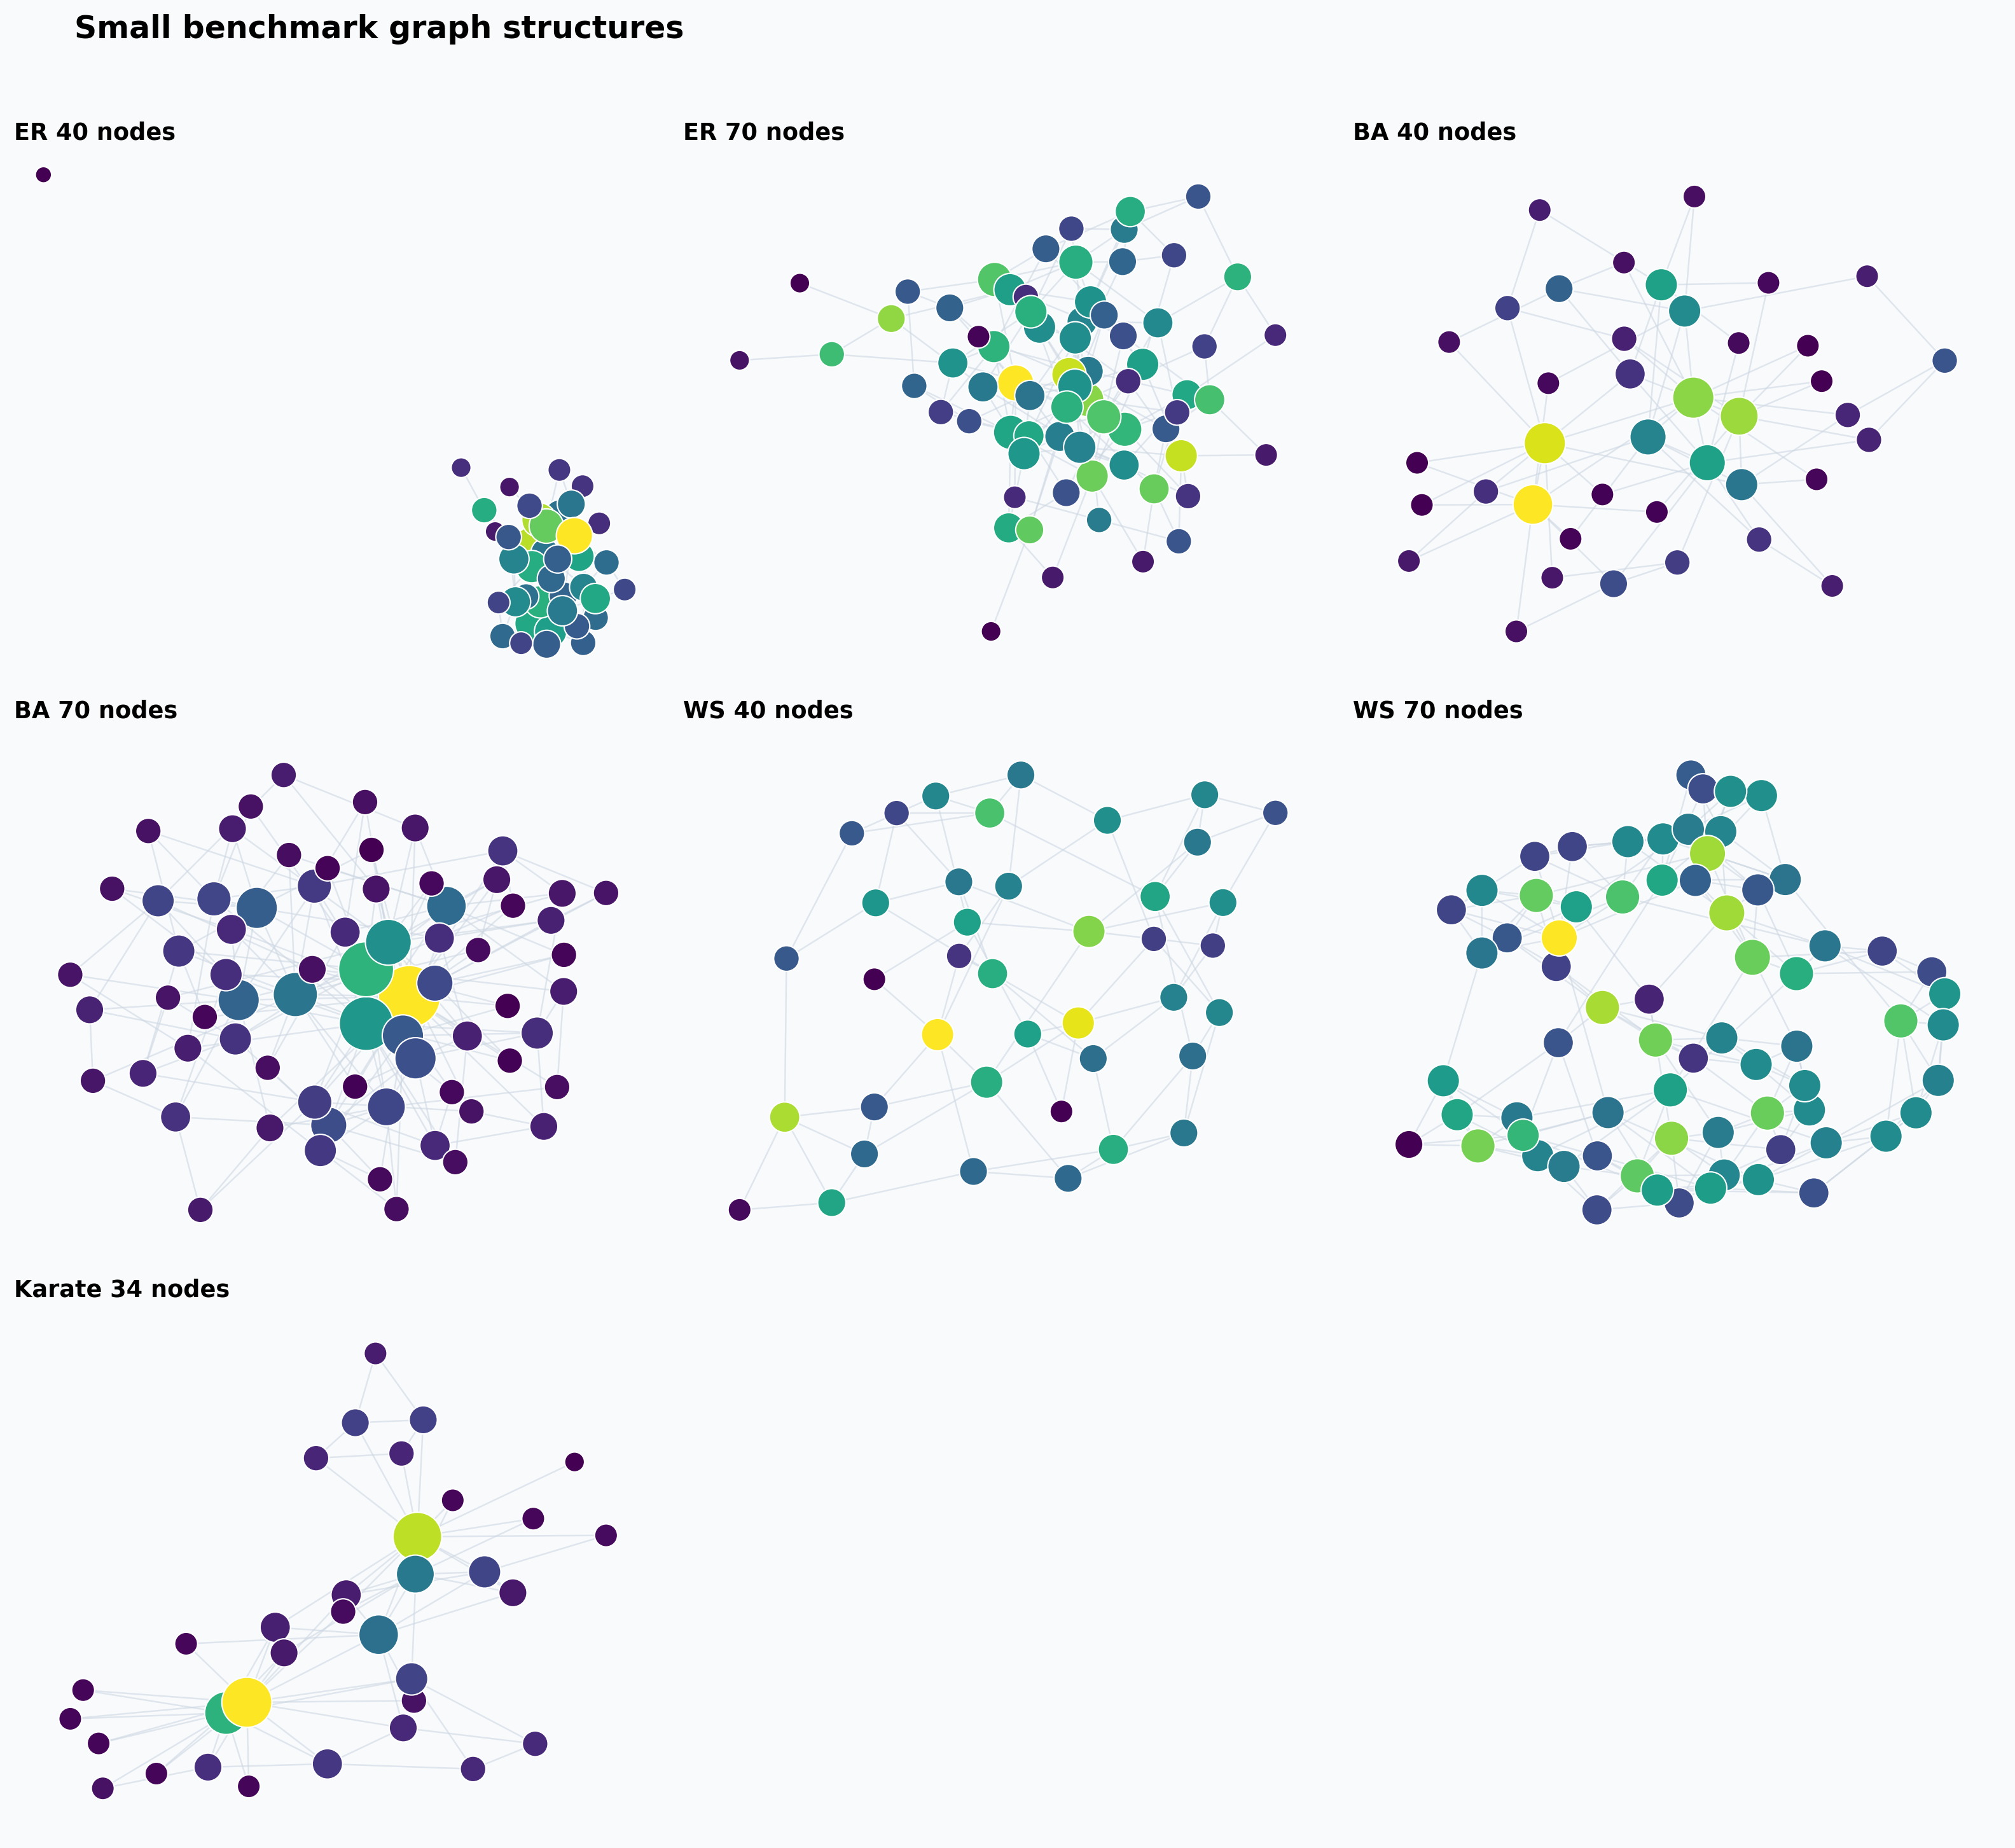
\includegraphics[height=8.2cm,keepaspectratio]{outputs/influence_maximization/figures/graphs/small_graph_structures.png}

  \vspace{0.16cm}
  \small Random, hub-heavy, small-world, and Karate Club graph structures expose different seed-selection behavior.
}
\end{column}

\begin{column}{0.350\textwidth}
\vspace{0pt}
\panel{Algorithmic Story}{
  \centering
  \begin{tikzpicture}[node distance=0.65cm and 0.70cm]
    \node[algo,text width=4.9cm] (simple) {Structure baselines\\Random, degree, PageRank};
    \node[algo,right=of simple,text width=5.0cm] (greedy) {Centralized greedy\\best MC marginal gain};
    \node[algo,right=of greedy,text width=4.9cm] (celf) {CELF\\lazy marginal refresh};
    \node[algo,below=1.08cm of greedy,text width=5.3cm] (dist) {GreeDI-style\\local candidates + coordinator};

    \draw[arrow] (simple) -- (greedy);
    \draw[arrow] (greedy) -- (celf);
    \draw[arrow] (greedy) -- (dist);

    \node[note,below=0.65cm of simple] (q1) {How strong are simple graph heuristics?};
    \node[note,below=0.65cm of dist] (q2) {How much quality survives limited communication?};
    \node[note,below=0.65cm of celf] (q3) {How many spread calls can submodularity save?};
    \draw[softarrow] (simple) -- (q1);
    \draw[softarrow] (dist) -- (q2);
    \draw[softarrow] (celf) -- (q3);
  \end{tikzpicture}
}

\vspace{0.36cm}
\panel{Distributed Candidate Sharing}{
  \centering
  \begin{tikzpicture}[node distance=0.33cm and 0.52cm]
    \node[local] (p1) {Partition 1\\local greedy};
    \node[local,below=of p1] (p2) {Partition 2\\local greedy};
    \node[local,below=of p2] (pm) {Partition \(m\)\\local greedy};
    \node[algo,right=0.78cm of p2,text width=4.55cm] (pool) {Union of top-\(q\) candidates};
    \node[algo,right=of pool,text width=4.25cm] (coord) {Coordinator greedy};
    \node[algo,right=of coord,text width=3.45cm] (seeds) {Final seeds};

    \draw[arrow] (p1.east) -- (pool.west);
    \draw[arrow] (p2.east) -- (pool.west);
    \draw[arrow] (pm.east) -- (pool.west);
    \draw[arrow] (pool) -- (coord);
    \draw[arrow] (coord) -- (seeds);
  \end{tikzpicture}

  \vspace{0.20cm}
  Each worker sends at most \(q\) candidate nodes. The coordinator searches only the merged candidate pool.
}

\vspace{0.36cm}
\panel{Experimental Protocol}{
  \begin{tabular}{@{}ll@{}}
    \toprule
    Graph families & Erdos-Renyi, Barabasi-Albert, Watts-Strogatz, Karate \\
    Large sizes & \(n\in\{50,100,200\}\), plus Karate \\
    Seed budget & \(k=10\) for synthetic large graphs, \(k=5\) for Karate \\
    Distributed sweep & \(m\in\{2,4,8\}\), \(q\in\{k,2k,5k\}\) \\
    Fair evaluation & final seed sets re-estimated with a common seed \\
    \bottomrule
  \end{tabular}
}

\vspace{0.36cm}
\begin{columns}[T,totalwidth=\linewidth]
  \begin{column}{0.48\linewidth}
    \resultcard{74.1\% fewer evaluations}{CELF vs. greedy}{Large-scale average: 266.2 vs. 1026.5 spread evaluations.}
  \end{column}
  \begin{column}{0.48\linewidth}
    \resultcard{83.5\% lower runtime}{CELF vs. greedy}{Large-scale average: 0.77s vs. 4.67s wall-clock time.}
  \end{column}
\end{columns}
\end{column}

\begin{column}{0.365\textwidth}
\vspace{0pt}
\panel{Large-Scale Evidence}{
  \begin{columns}[T,totalwidth=\linewidth]
    \begin{column}{0.43\linewidth}
      \centering
      \begin{tabular}{lrrrr}
        \toprule
        Method & Spread & Ratio & Time & Eval. \\
        \midrule
        Random & 31.59 & 0.791 & 0.00s & 1.0 \\
        W. Degree & 43.71 & 1.066 & 0.01s & 1.0 \\
        PageRank & 35.19 & 0.893 & 0.00s & 1.0 \\
        Greedy & 40.43 & 1.000 & 4.67s & 1026.5 \\
        CELF & 40.05 & 0.988 & 0.77s & 266.2 \\
        \bottomrule
      \end{tabular}
    \end{column}
    \begin{column}{0.54\linewidth}
      \begin{itemize}
        \item CELF nearly preserves greedy spread but sharply cuts spread calls.
        \item Weighted degree is not a weak baseline under weighted-cascade probabilities.
        \item Distributed quality remains competitive, but communication cost rises quickly.
      \end{itemize}
    \end{column}
  \end{columns}
}

\vspace{0.36cm}
\panel{Case-Level Results}{
  \centering
  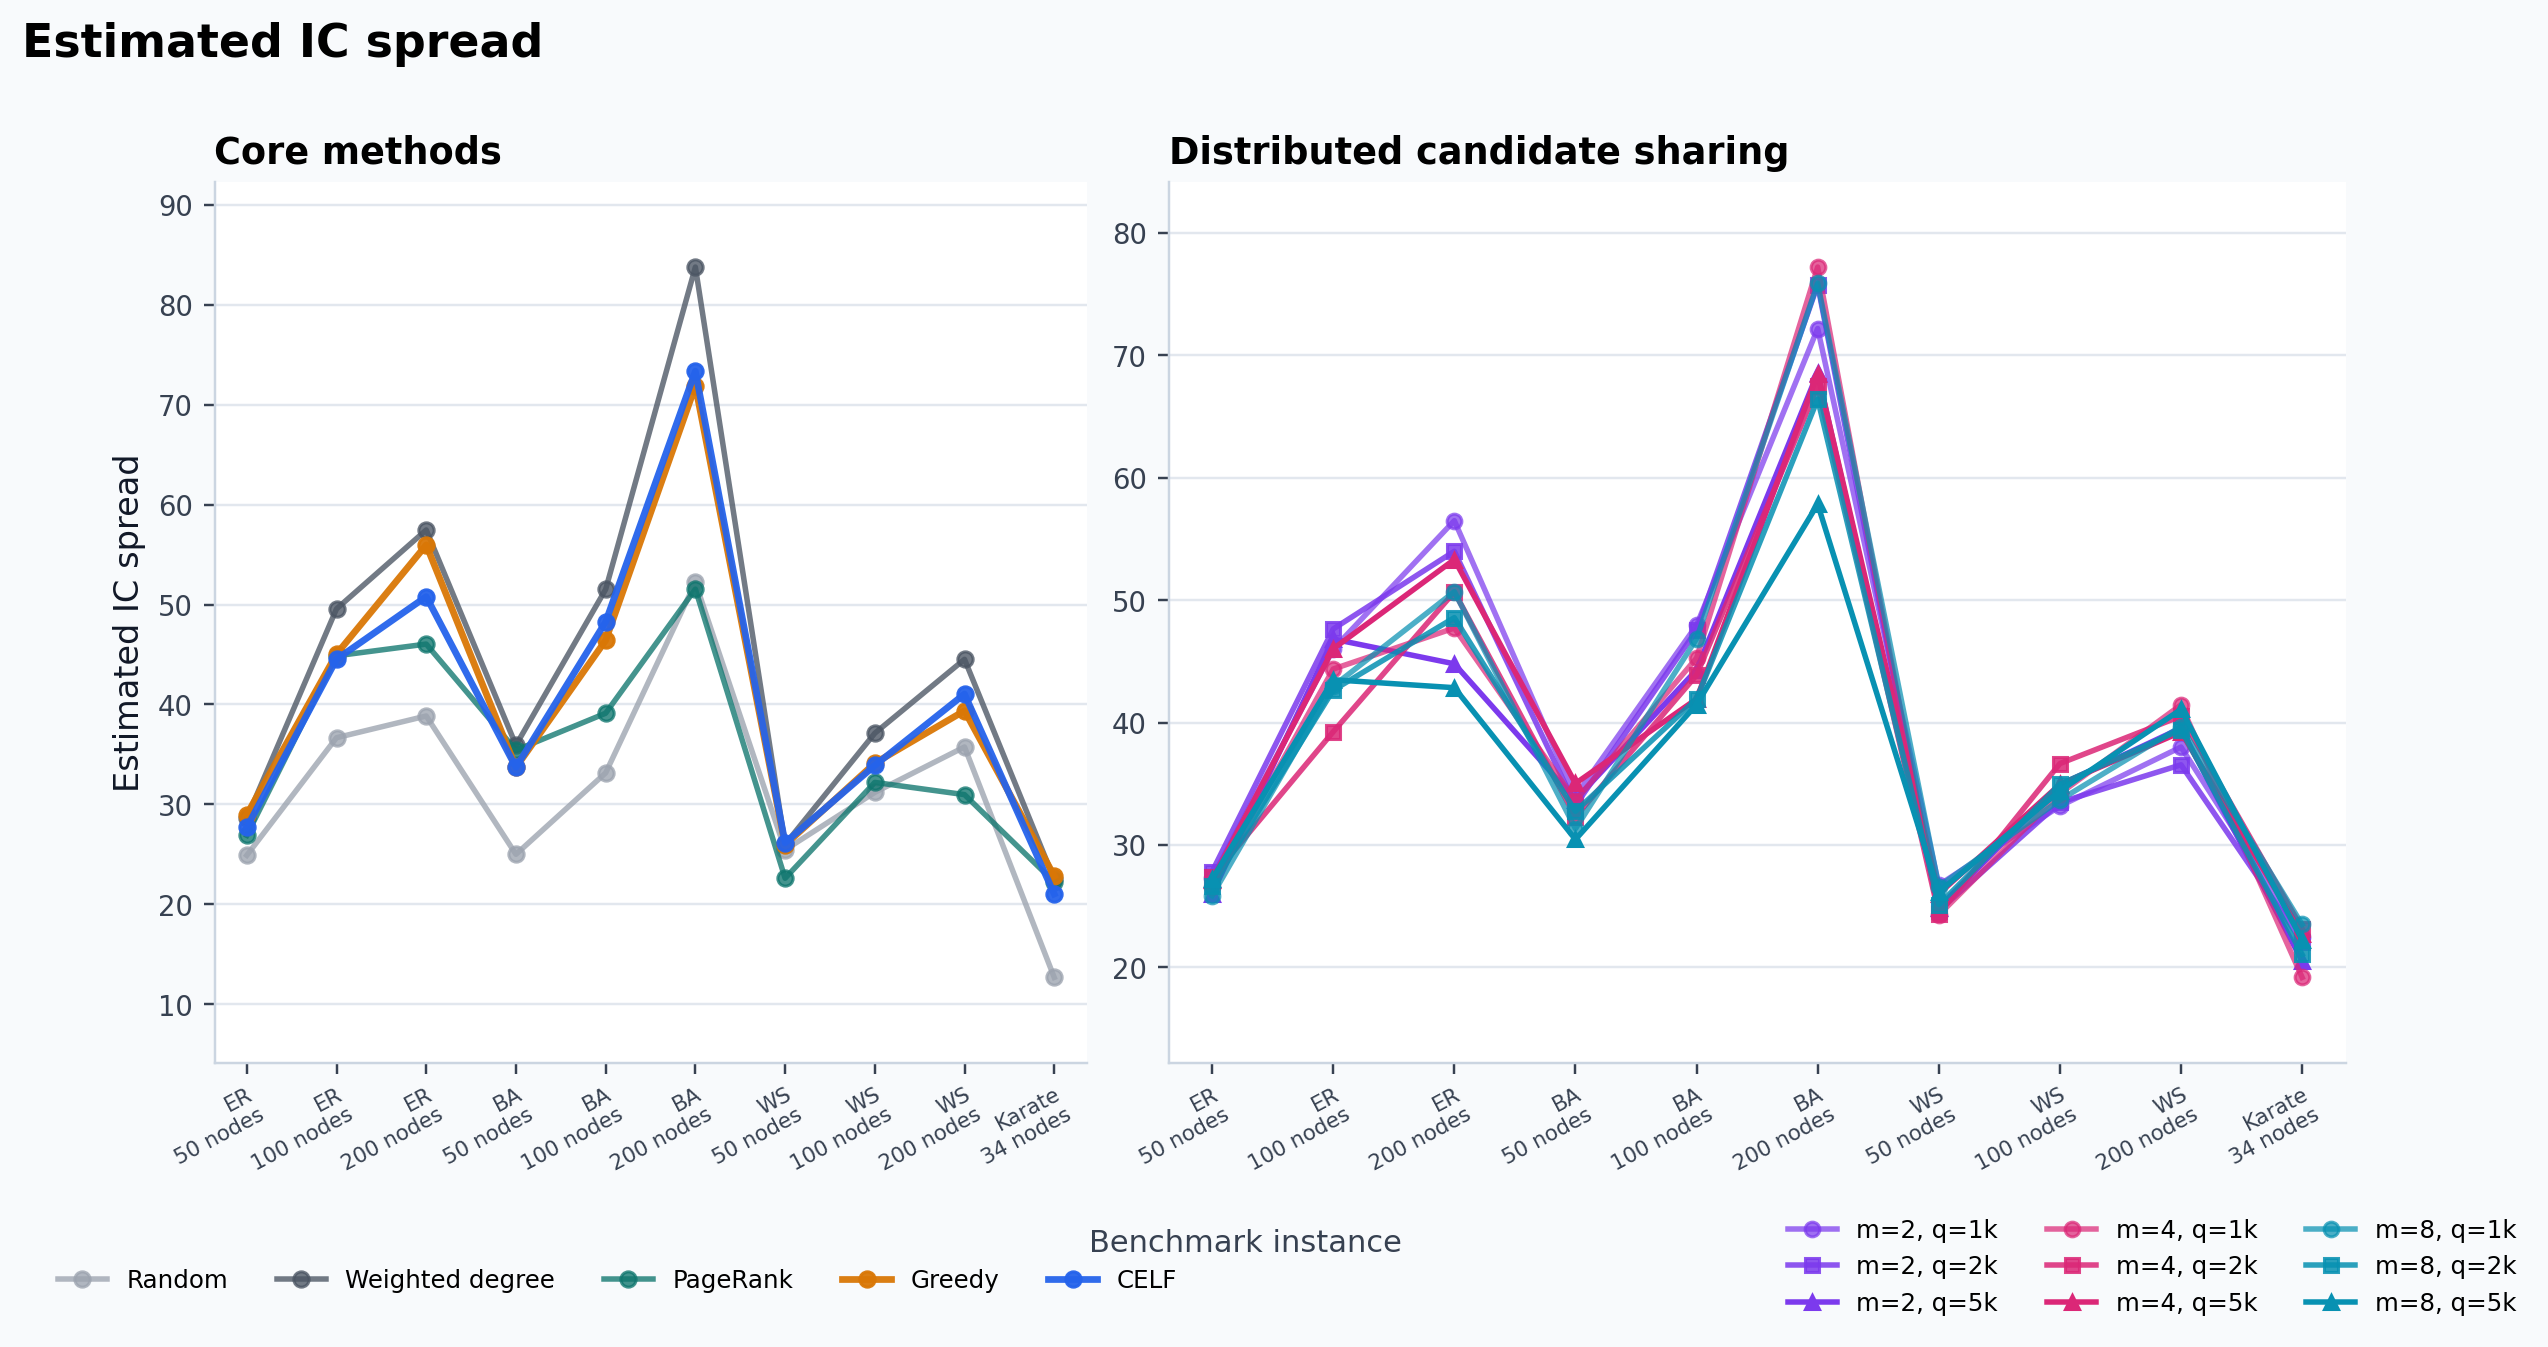
\includegraphics[width=0.493\linewidth]{outputs/influence_maximization/figures/estimated_spread_large.png}
  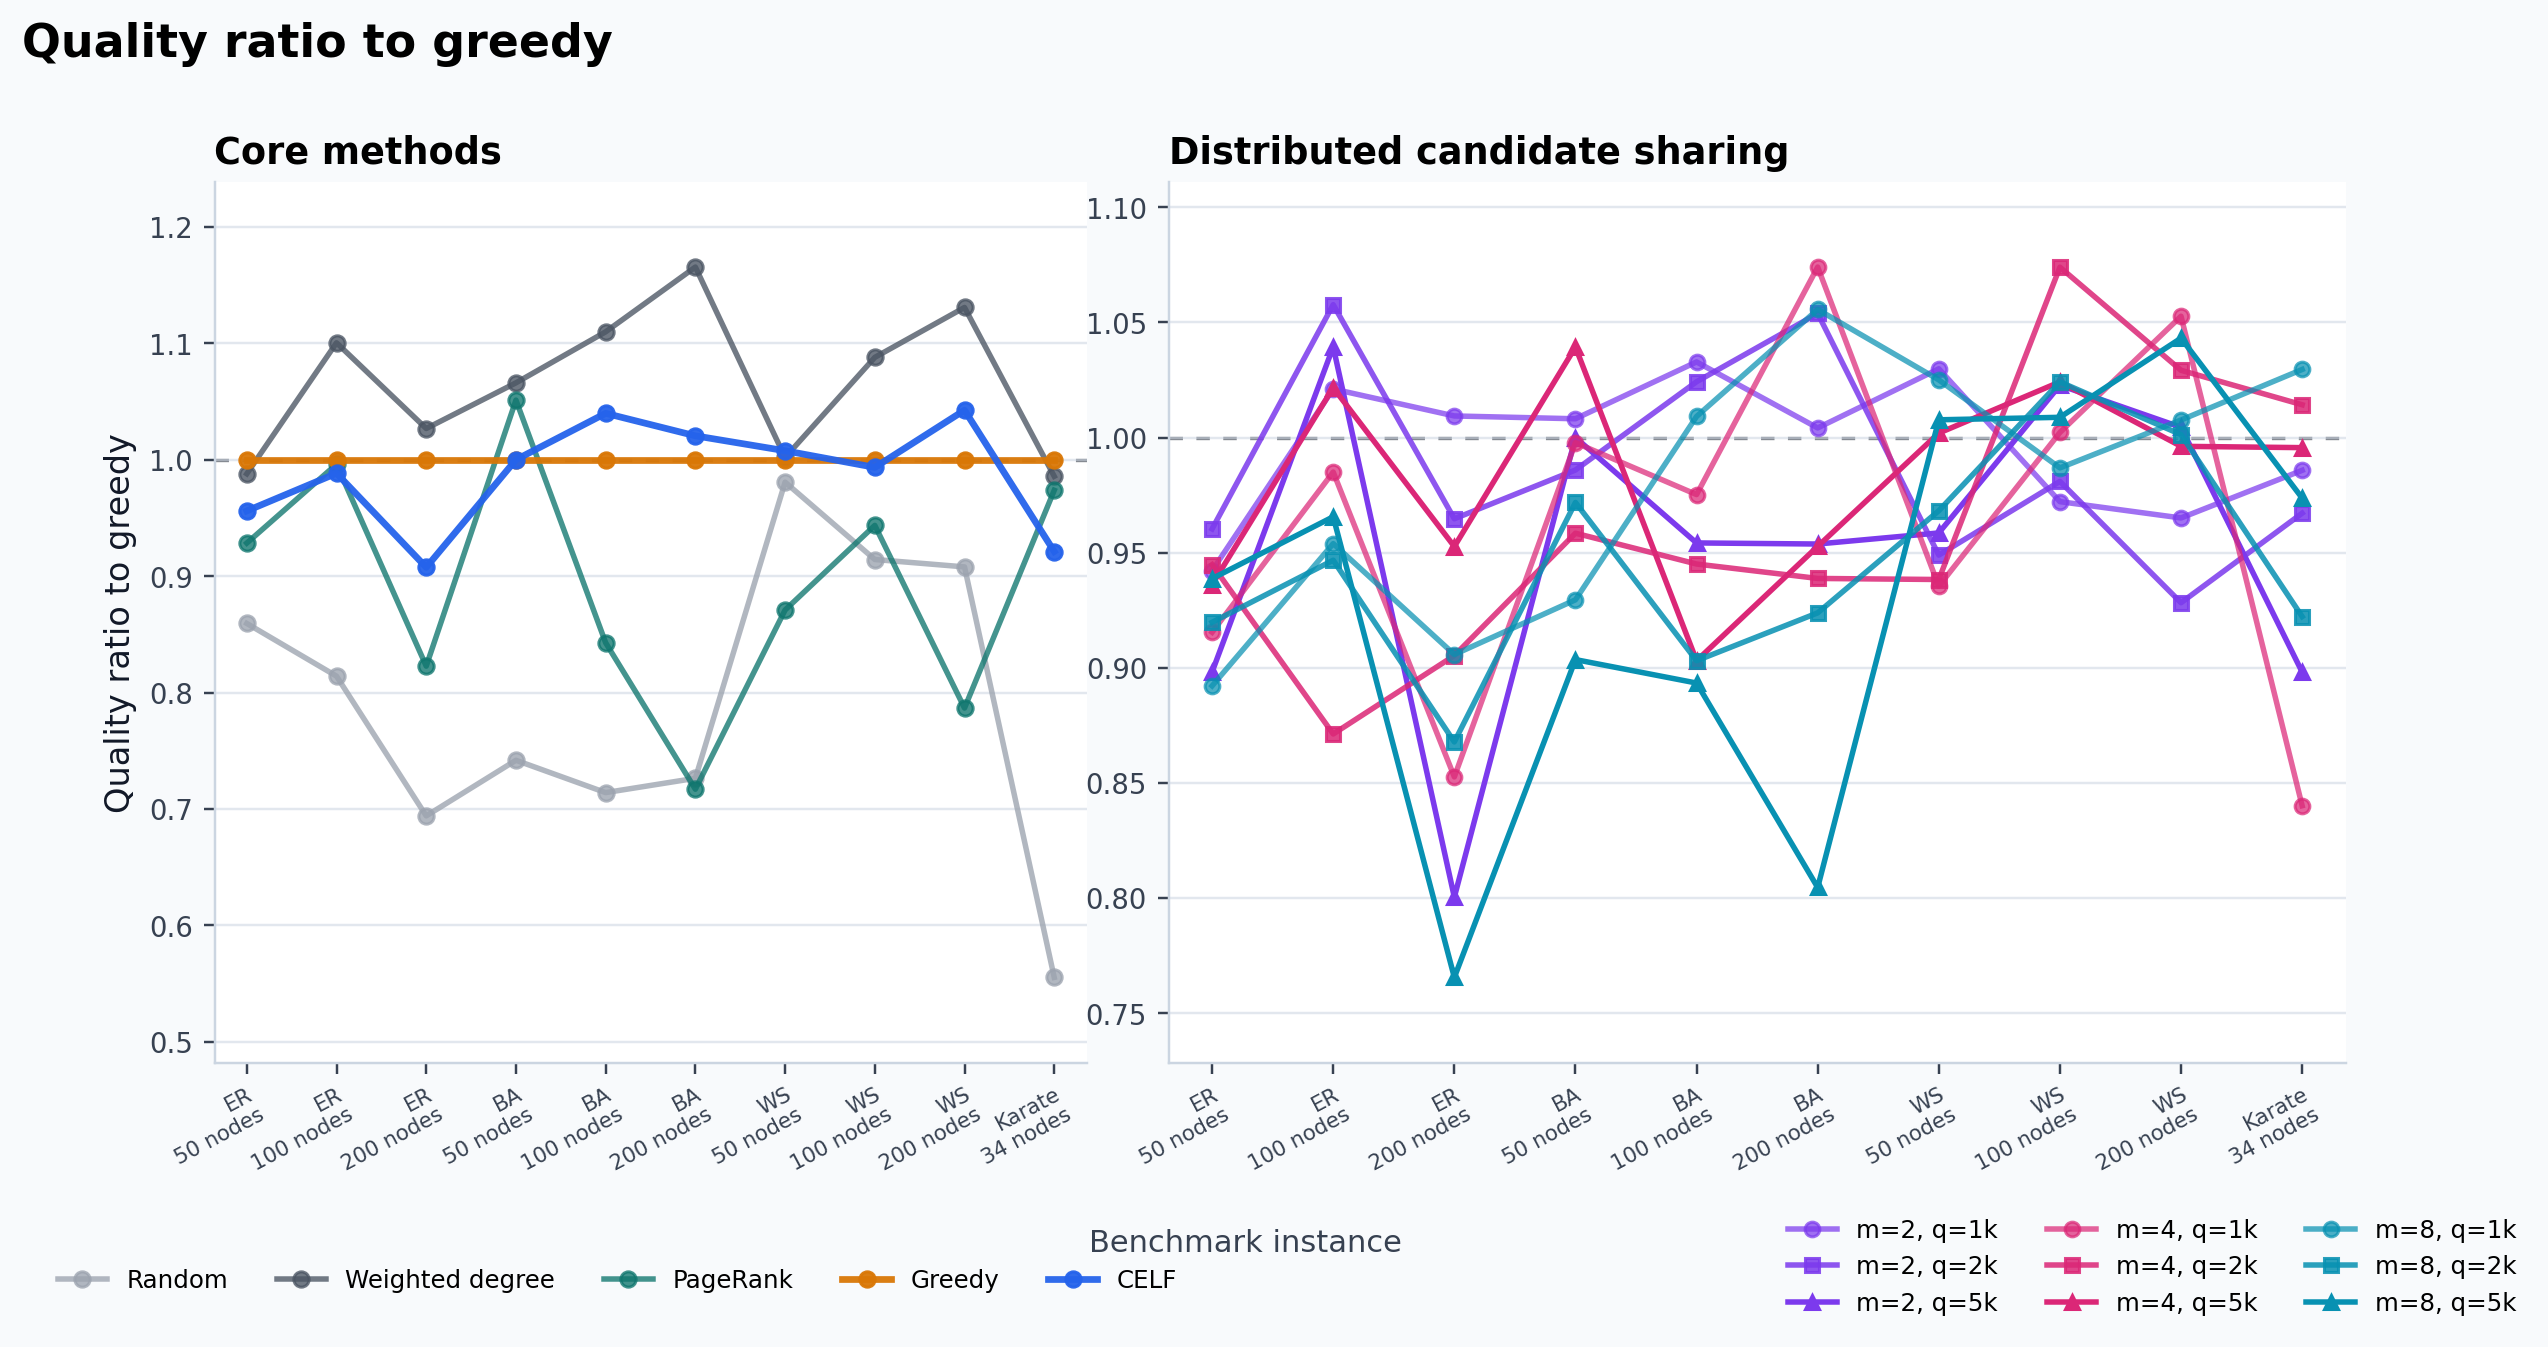
\includegraphics[width=0.493\linewidth]{outputs/influence_maximization/figures/quality_ratio_to_greedy_large.png}

  \vspace{0.28cm}
  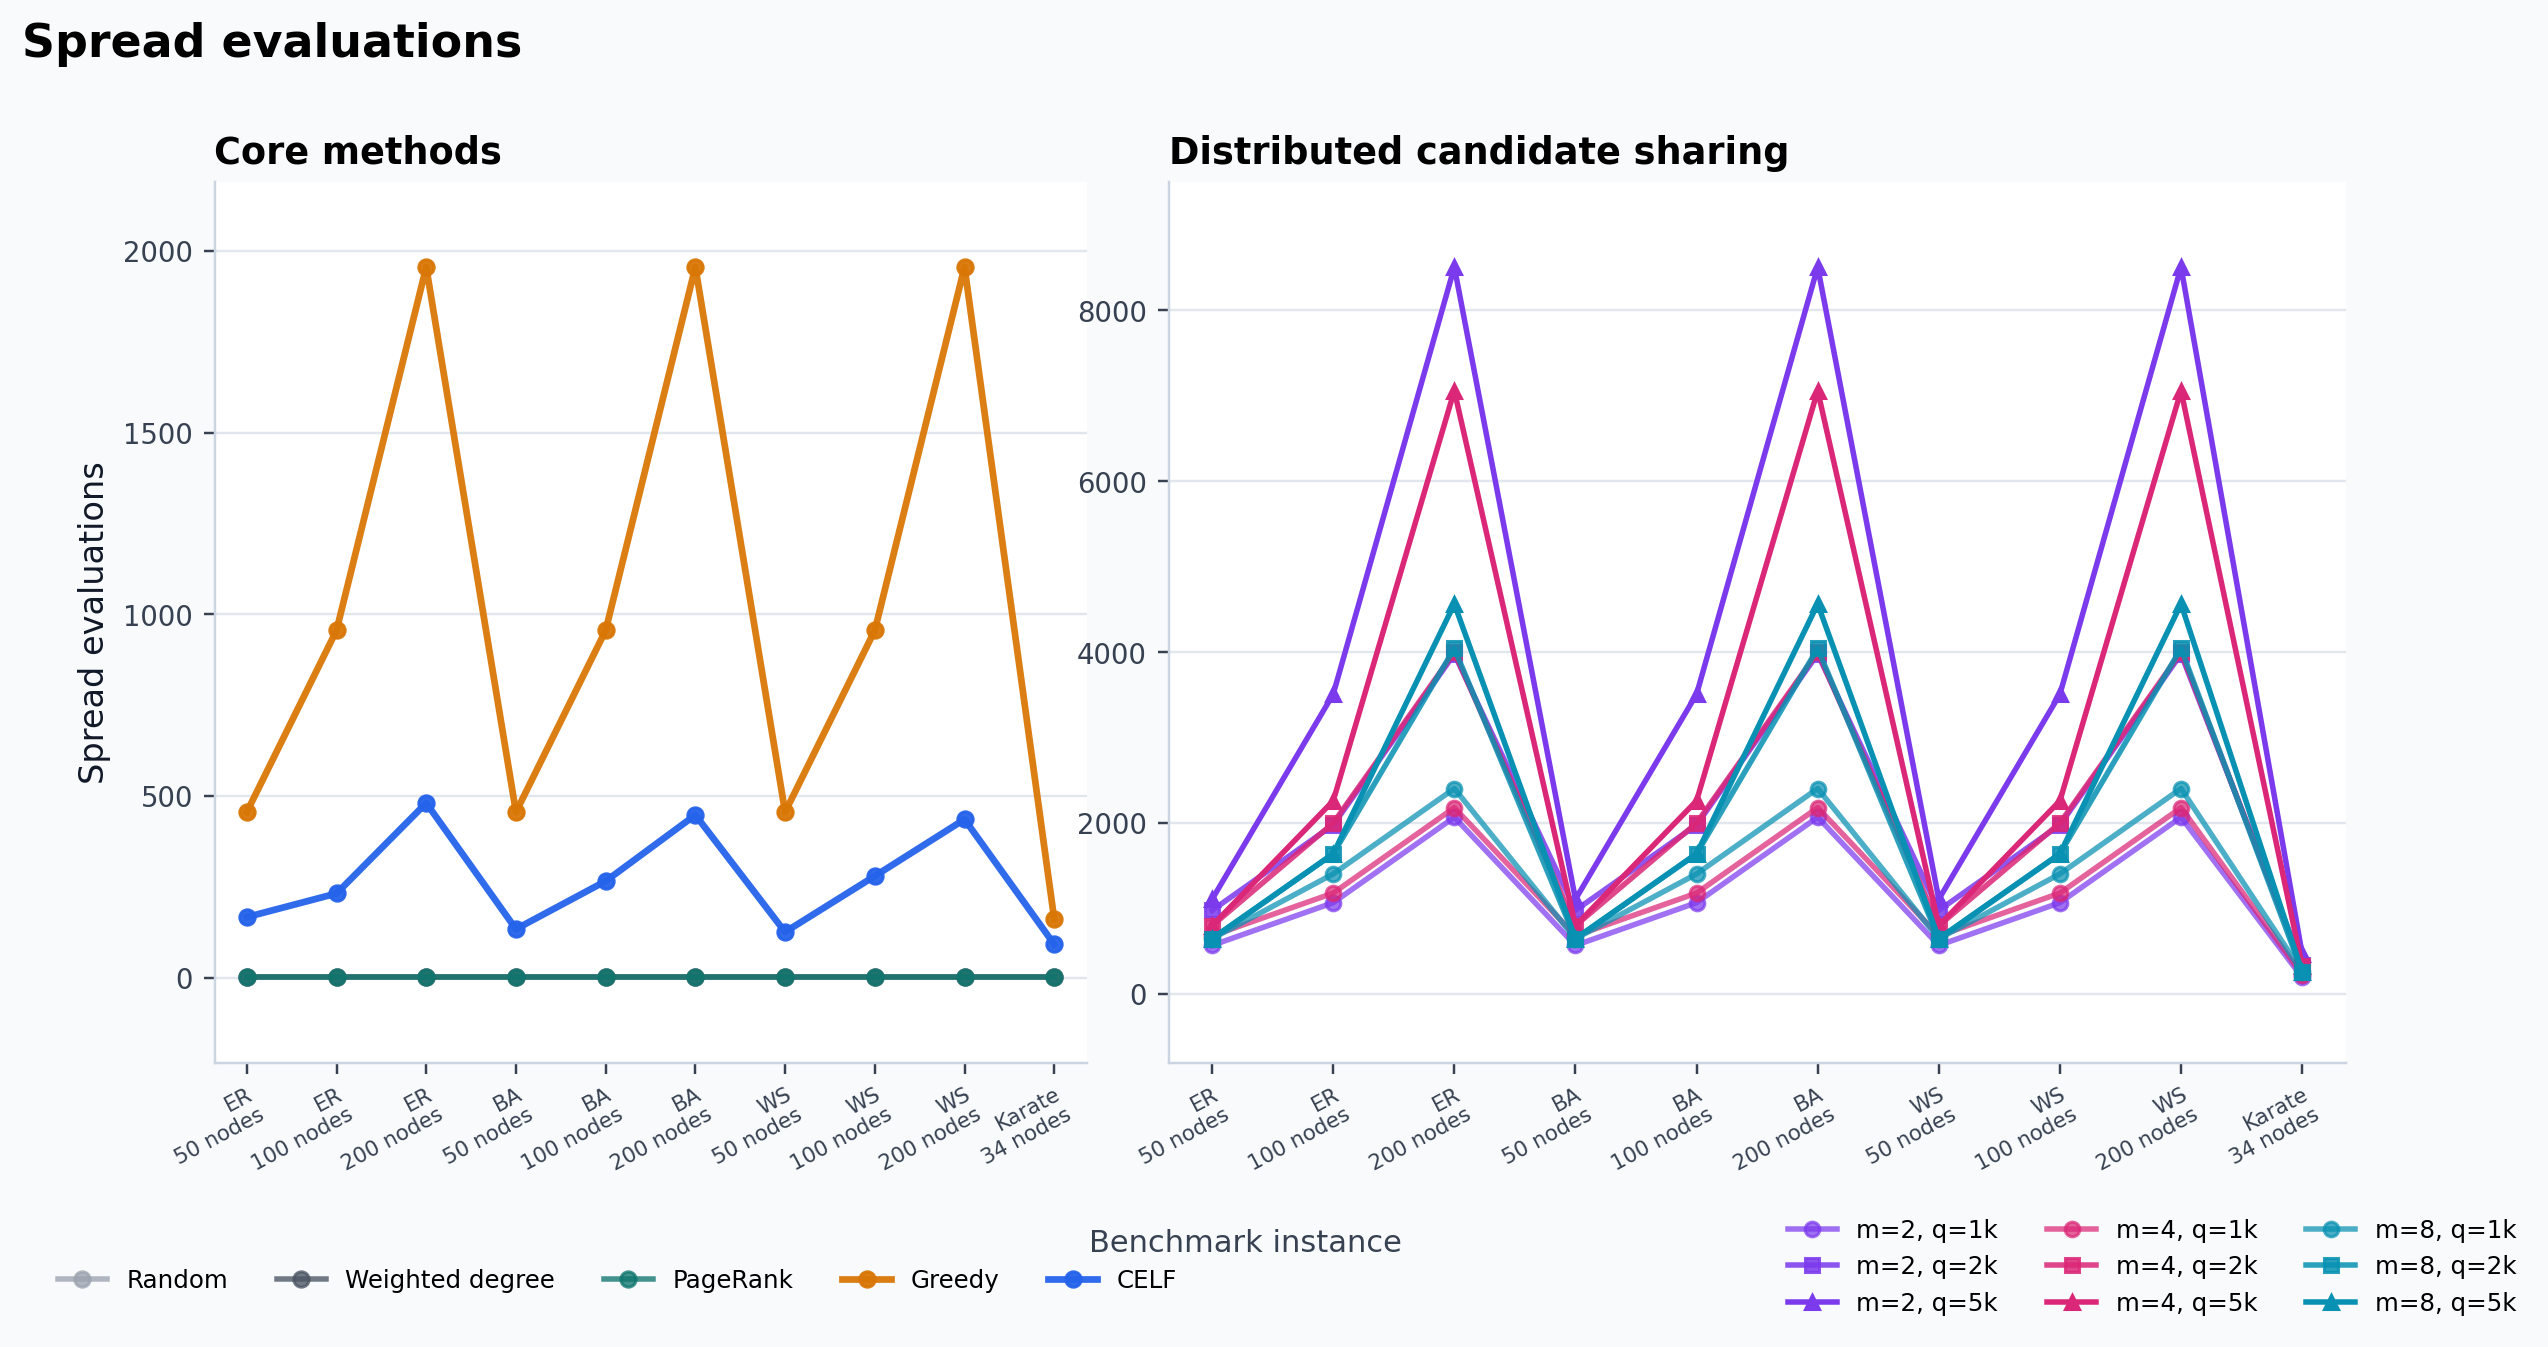
\includegraphics[width=0.493\linewidth]{outputs/influence_maximization/figures/spread_evaluations_large.png}
  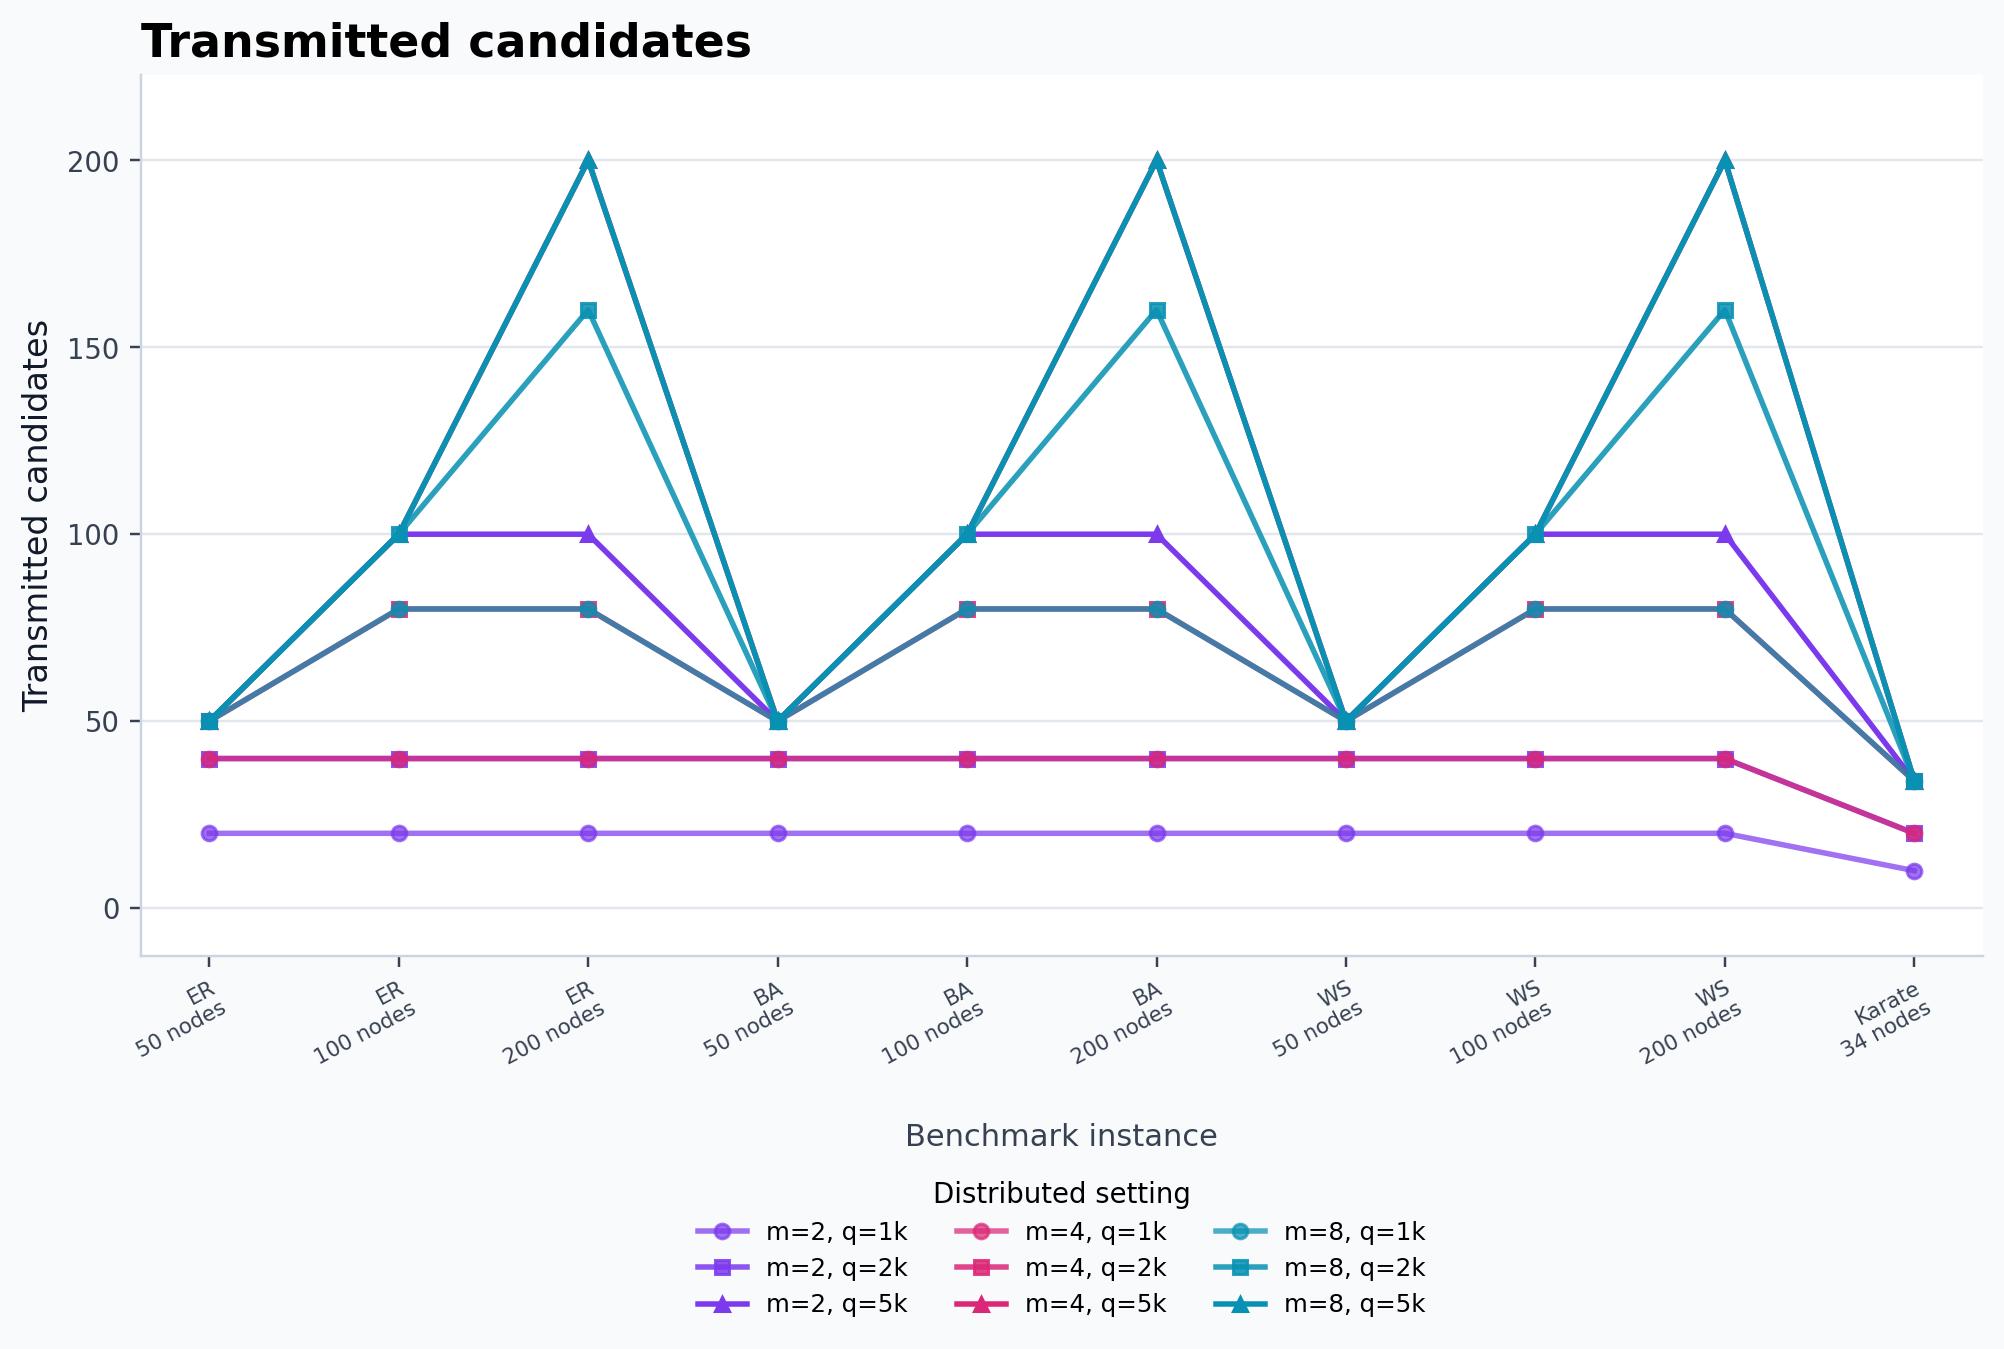
\includegraphics[width=0.493\linewidth]{outputs/influence_maximization/figures/transmitted_candidates_large.png}
}

\vspace{0.36cm}
\panel{Communication Tradeoff}{
  \begin{columns}[T,totalwidth=\linewidth]
    \begin{column}{0.42\linewidth}
      \centering
      \begin{tabular}{lrrrr}
        \toprule
        Budget & Ratio & Time & Eval. & Cand. \\
        \midrule
        \(q=k\) & 0.980 & 1.58s & 1242.4 & 41.1 \\
        \(q=2k\) & 0.965 & 3.36s & 2037.2 & 66.9 \\
        \(q=5k\) & 0.955 & 6.48s & 3044.4 & 98.4 \\
        \bottomrule
      \end{tabular}
    \end{column}
    \begin{column}{0.54\linewidth}
      Bigger candidate budgets transmit more nodes and trigger more evaluations. In this noisy course-scale setting, quality does not improve monotonically with \(q\).
    \end{column}
  \end{columns}
}

\vspace{0.36cm}
\panel{Takeaways}{
  \begin{itemize}
    \item Submodularity gives the project a principled greedy baseline.
    \item CELF is the clearest algorithmic improvement: it keeps the target but removes redundant evaluations.
    \item Communication-limited candidate sharing changes the cost model: less global search, more sensitivity to partitions and Monte Carlo noise.
  \end{itemize}
}
\end{column}

\end{columns}

\vspace{0.50cm}
\begin{beamercolorbox}[wd=\textwidth,sep=0.34cm,rounded=true]{smallpanel}
  \begin{columns}[T,totalwidth=\textwidth]
    \begin{column}{0.31\textwidth}
      \textbf{Implementation.}
      IC simulation, greedy selection, CELF, and distributed candidate sharing are implemented as separate modules.
    \end{column}
    \begin{column}{0.31\textwidth}
      \textbf{Run command.}
      \texttt{python src/experiments.py --scale large --seed 7 --simulations 40}
    \end{column}
    \begin{column}{0.31\textwidth}
      \textbf{Scope.}
      This is a course-scale reproduction of algorithmic mechanisms, not a full IMM/RIS or production distributed system.
    \end{column}
  \end{columns}
\end{beamercolorbox}

\vspace{0.28cm}
\begin{beamercolorbox}[wd=\textwidth,sep=0.20cm,rounded=true]{takeaway}
  \centering
  {\scriptsize References: Kempe, Kleinberg, and Tardos, KDD 2003; Nemhauser, Wolsey, and Fisher, Mathematical Programming 1978; Leskovec et al., KDD 2007; Mirzasoleiman et al., NeurIPS 2013.}
\end{beamercolorbox}

\end{frame}
\end{document}
